\documentclass{scrartcl}
\usepackage[utf8]{inputenc}
\usepackage[T1]{fontenc}
\usepackage[a4paper]{geometry}
\usepackage{graphicx}
\usepackage{hyperref}
\usepackage{float}
\usepackage{mathtools}
\usepackage{textcomp}
\usepackage{gensymb}
\usepackage[ngerman]{babel}
\usepackage{epstopdf}
\usepackage{titlesec}
\renewcommand{\arraystretch}{1.3}
\setcounter{secnumdepth}{5}
\setcounter{tocdepth}{5}
\makeatletter
\renewcommand\paragraph{\@startsection{paragraph}{4}{\z@}%
  {-3.25ex\@plus -1ex \@minus -.2ex}%
  {1.5ex \@plus .2ex}%
  {\normalfont\normalsize\bfseries}}
\newcommand*{\tline}{%
  \ifmeasuring@
  % first measuring run
  \else
  % second run
  % \typeout{\meaning\maxcolumn@widths}% debug info
  \ifodd\column@
  \expandafter\rlap
  \else
  \expandafter\llap
  \fi
     {%
       \vrule height-1ex depth \dimexpr1ex+.4pt\relax width
       \ifcase\numexpr\column@+1\expandafter\relax
       \maxcolumn@widths
       \fi
     }%
     \fi
}
\makeatother
\restylefloat{table}
\newcommand{\mytitle}{Übung 1}
\hypersetup{
  colorlinks=true,
  linkcolor=blue,
  pdftitle=\mytitle,
  pdfauthor={Fabian Nedoluha, Stefan Hermeter},
}
\begin{document}
\title{\mytitle:Arrays und Strings}
\subtitle{String verarbeitung}
\date{\today}
\author{Stefan Hermeter \texttt{\href{mailto:stefan.hermeter@gmx.at}{stefan.hermeter@gmx.at}}\\
  Klasse: 5ABETi\\
  Schuljahr: 2015/16, 28. November}
\pagenumbering{gobble}
\maketitle
\pagenumbering{roman}
\newpage
\tableofcontents
\listoffigures
\newpage
\pagenumbering{arabic}
\section{Aufgabenstellung}
\subsection{Erster Teil}
Schreiben Sie ein Programm namens SkalarProd, welches das Skalarprodukt zweier n-dimensionaler Vektoren berechnet, welches die Summe zweier Matrizen bildet und welches eine nxm- und eine mxn-Matrix multipliziert\\

\subsection{Zweiter Teil}
Erstellen Sie eine eigene String-Bibliothek mit dem Namen 'myString.h'. Erstellen Sie ein Programm myStrings.c für das Testen der Funktionen mit entsprechenden Ein- und Ausgabeoperationen. Es sollen alle Funktionen bzw. deren richtige Funktionalität sichtbar sein

%% Programmablauf
\section{Programmablaufplan}
\subsection{Erster Teil: Schema Programmablauf}
\begin{figure}[H]
  \centering
  \includegraphics[width=0.8\linewidth]{images/Flussdiagramm_erster_teil.eps}
  \caption{Programmablauf MatAdd MatMult}
  \label{fig:digraph}
\end{figure}
\subsection{Zweiter Teil: Schema Programmablauf}
\begin{figure}[H]
  \centering
  \includegraphics[width=0.8\linewidth]{images/Flussdiagramm_zweiter_teil.eps}
  \caption{Programmablauf myString.h}
  \label{fig:digraph}
\end{figure}

%% Resourcen | Libraries
\section{Resourcen Erster Teil}
\subsection{Erster Teil}
\subsubsection{Sourcecode-Files}
\begin{itemize}
\item SkalarProd.c
\end{itemize}

\subsubsection{Verwendete Libraries}
\begin{itemize}
\item stdio.h
\item stdlib.h
\item time.h
\end{itemize}

\subsection{Zweiter Teil}
\subsubsection{Sourcecode-Files}
\begin{itemize}
\item test\_prog.c
\end{itemize}

\subsubsection{Verwendete Libraries}
\begin{itemize}
\item stdio.h
\item stdlib.h
\item myString.h
\end{itemize}

%% Testergebnisse 
\section{Testergebnisse}

\subsection{Test: Erster Teil}
\begin{figure}[H]
  \centering
  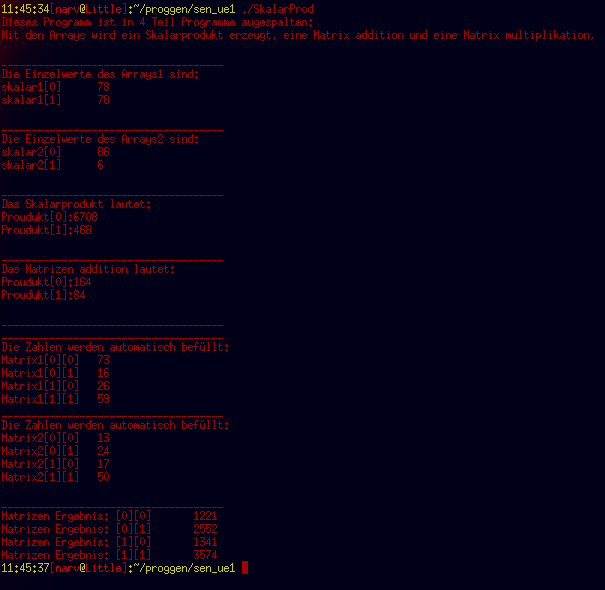
\includegraphics[width=0.9\linewidth]{images/test1.png}
  \caption{Testlauf 1}
  \label{fig:digraph}
\end{figure}

\begin{figure}[H]
  \centering
  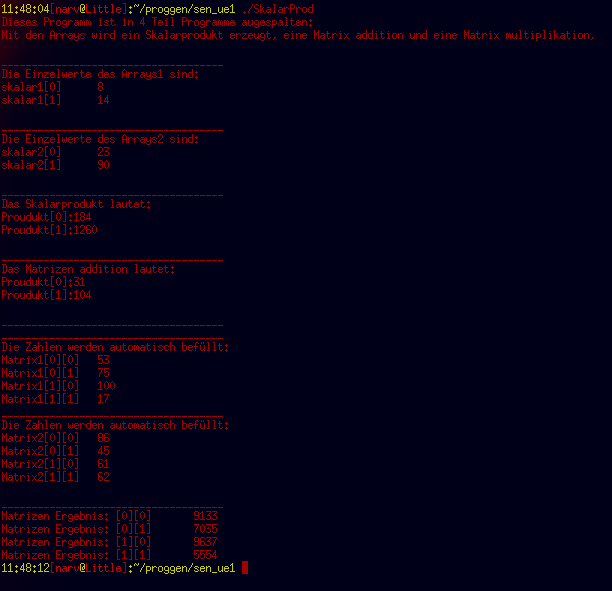
\includegraphics[width=0.9\linewidth]{images/test2.png}
  \caption{Testlauf 2}
  \label{fig:digraph}
\end{figure}

\subsection{Test: Zweiter Teil}
\begin{figure}[H]
  \centering
  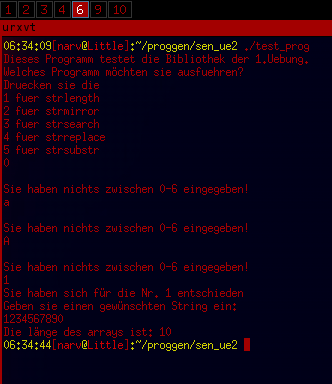
\includegraphics[width=0.9\linewidth]{images/test_prog1.png}
  \caption{myString.h test strlength}
  \label{fig:digraph}
\end{figure}

\begin{figure}[H]
  \centering
  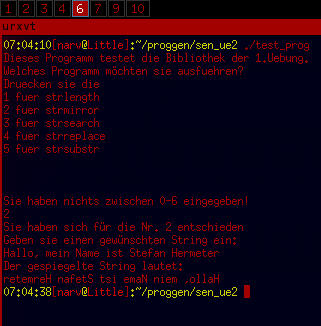
\includegraphics[width=0.9\linewidth]{images/test_prog2.png}
  \caption{myString.h test strmirror}
  \label{fig:digraph}
\end{figure}

\begin{figure}[H]
  \centering
  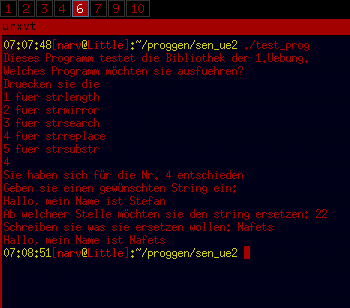
\includegraphics[width=0.9\linewidth]{images/test_prog4.png}
  \caption{myString.h test strreplace}
  \label{fig:digraph}
\end{figure}

\end{document}
